\documentclass[english, a4paper, 12pt, twoside]{article}

% -------------- Setup, do not change these ---------------
\usepackage{textcomp}
\usepackage[T1]{fontenc, url}
\usepackage[utf8]{inputenc}
\usepackage{titlesec}
\setcounter{secnumdepth}{4}
\usepackage{multirow}

\usepackage{adjustbox}
\usepackage{graphicx}
\usepackage{amsmath, amssymb, amsthm} % Mathematical packages
\usepackage{parskip} % Removing indenting in new paragraphs
\urlstyle{sf}
\usepackage{color}
\usepackage{subcaption}
\usepackage{appendix}
\usepackage{chngcntr} % needed for correct table numbering
\counterwithin{table}{section} % numbering of tables
\counterwithin{figure}{section} % numbering of figures
\numberwithin{equation}{section} % numbering of equations
\hyphenpenalty=100000 % preventing splitting of words
\sloppy
\raggedbottom
\usepackage{xparse,nameref}
\usepackage[bottom]{footmisc} % Fotnotes are fixed to bottom of page

% --------- You can edit from this point on --------


% ----- Appearance and language -----
\usepackage[english]{babel} % document language
\graphicspath{./img/} % path to images
\usepackage[margin=2.54cm]{geometry} % sets margins for the document
\usepackage{setspace}
\linespread{1} % line spread for the document
\usepackage{microtype}


% ----- Sections -----
\titleformat*{\section}{\LARGE\bfseries} % \section heading
\titleformat*{\subsection}{\Large\bfseries} % \subsection heading
\titleformat*{\subsubsection}{\large\bfseries} % \subsubsection heading
% next three lines creates the \paragraph command with correct heading
\titleformat{\paragraph}
{\normalfont\normalsize\bfseries}{\theparagraph}{1em}{}
\titlespacing*{\paragraph}
{0pt}{3.25ex plus 1ex minus .2ex}{1.5ex plus .2ex}


% ----- Figures and tables -----
\usepackage{fancyhdr}
\usepackage{subfiles}
\usepackage{array}
\usepackage[rightcaption]{sidecap}
\usepackage{wrapfig}
\usepackage{float}
\usepackage[labelfont=bf]{caption} % bold text for captions
\usepackage[para]{threeparttable} % fancy tables, check these before you use them
\usepackage{url}
\usepackage[table,xcdraw]{xcolor}
\usepackage{makecell}
\usepackage{hhline}

\usepackage[breaklinks=true,colorlinks=true,linkcolor=black,urlcolor=blue,citecolor=blue]{hyperref}
% ----- Sources -----

%\bibliographystyle{apa} % citation and reference list style
%\def\biblio{\clearpage\bibliographystyle{apa}\bibliography{References.bib}} % defines the \biblio command used for referencing in subfiles - DO NOT CHANGE


% ----- Header and footer -----
\pagestyle{fancy}
\fancyhead[RO,LE]{\thepage} % page number on right for odd pages and left for even pages in the header
\fancyhead[RE,LO]{\nouppercase{\rightmark}} % chapter name and number on the right for even pages and left for odd pages in the header
%\renewcommand{\headrulewidth}{0pt} % sets thickness of header line
\fancyfoot{} % removes page number on bottom of page


% ----- Header of the frontpage -----
\fancypagestyle{frontpage}{
	\fancyhf{}
	\renewcommand{\headrulewidth}{0pt}
	\renewcommand{\footrulewidth}{0pt}
	\vspace*{1\baselineskip}

	%\fancyhead[R]{Norwegian School of Economics
	%\linebreak       Bergen, Fall 2018\vspace*{5\baselineskip}}
	\fancyhead[C]{ 
\includegraphics[width=3.5in]{img/logo}}
}


% ----- Document starts here -----
\begin{document}

%\def\biblio{} % resets the biblio command, if not here a new reference list will be produced after every chapter
{\setstretch{1.5}

\begin{titlepage}

 \newgeometry{top=1 in, bottom=1 in, left=1 in, right= 1 in}

 \thispagestyle{frontpage}

 \begin{center}

   \vspace*{6\baselineskip}


   {\Huge \textbf{Fancy title with many fancy words\\}}

   

       \vspace*{1,5\baselineskip}


   \vspace{1,5\baselineskip}

   \large{A master’s thesis submitted to the faculty of mathematics, computer science and physics, of the University of Innsbruck\\ in partial fulfillment of the requirements for the degree of\\\vspace{1,2\baselineskip}\textbf{Master of Science (MSc)} \\\vspace{1,2\baselineskip}carried out at the Institute of Experimental Physics under the supervision of}\\
   \large{o.Univ.-Prof.  Dr.  Rainer Blatt,}\\
   \large{Dr. Ben Lanyon}\\
    \vspace{1,2\baselineskip}
   \large{Presented by\\}
   \huge{\textbf{Marco Canteri}}\\
   

 \end{center}

\end{titlepage}

}
\restoregeometry % restores the margins after frontpage
%\nocite{*} % uncomment if you want all sources to be printed in the reference list, including the ones which are not cited in the text

\pagenumbering{gobble} % suppress page numbering
\thispagestyle{plain} % suppress header
\clearpage\mbox{}\clearpage % add blank page

\pagenumbering{roman} % starting roman page numbering
\newpage

\section*{Abstract}
I swear I did something

\newpage


\newpage
\tableofcontents

\newpage
\listoffigures

\newpage
\addtocontents{toc}{\protect\setcounter{tocdepth}{4}} % sets depth of toc to 4, 1.1.1.1
\pagenumbering{arabic} % Starting arabic page numbering
\setcounter{page}{1} % sets pagecounter to 1

\section{Introduction} % section/chapter name

- Quantum computing/quantum networking \\
- Experiment context\\
- Master thesis project\\
- Outline\\

\section{Theoretical framework}
\subsection{Quantum logic with trapped ions}
\subsubsection{Quantum computer and quantum gates}
- Qubit\\
- Quantum operations\\
\subsubsection{Ion qubits and laser-ion interactions}
- 2 level atom scheme\\
- Model of laser-ion interaction: rabi flops, AC stark shift
\subsection{Quantum networking with trapped ions}
\subsubsection{General introduction}
- Nodes, interface, link, protocols\\
- logic, memory, interface, Bell pairs, purification, multi-mode
- Distributed entanglement
\subsubsection{Cavity QED}
- Simple model atom in cavity: g,gamma, k
\subsection{Basics of ion trapping}
\subsubsection{Linear Paul trap}
- How a Paul trap works\\
- micromotion?
\subsubsection{Ion strings}
We have seen that the potential inside the trap can be described as an harmonic potential. It is then possible to calculate the ion separation between $N$ ion loaded in the trap. This will give us an idea of how narrowly the beam should be focused and will set an appropriate problem spatial scale.\\
We will consider only the $z$ direction where the ions are weakly confined and will form a string. The harmonic potential is then given by
\begin{equation}
V = \sum_{i=0}^N \frac{1}{2}M\omega^2z_i^2 + \sum_{i\neq j}^N\frac{Z^2e^2}{8\pi \epsilon_0}\frac{1}{|z_i-z_j|}
\end{equation}
The equilibrium position can be found at the minima of the potential, i.e. where the first derivative zeros
\begin{equation}
\frac{\partial V}{\partial z_i} = 0 \implies u_i - \sum_{j\neq i}^{N} \frac{1}{(u_i-u_j)^2}= 0,
\end{equation}
where we defined the dimensionless quantity $u_i = z_i/l$ and $l^3 = \displaystyle\frac{Z^2 e^2 }{4\pi \epsilon_0 M\omega^2}$.
The last equations can be solved analytically only for 2 or 3 ions.
According to \cite{ion_spacing}
\subsection{Laser beam}
\subsubsection{Gaussian beams}
- Introduction to import quantities, like FWHM, focus, waist!
\subsubsection{Diffraction limit}
- To search whats limiting the diffraction, (lambda/2)
\subsubsection{Beam stearing via AOD's}
- How AODs work, simple Model\\
- Introduce diffraction efficiency, bandwidth
\subsection{Addressing system overview and requirements}
- First look at setup and requirements

\begin{figure}[H]
\centering
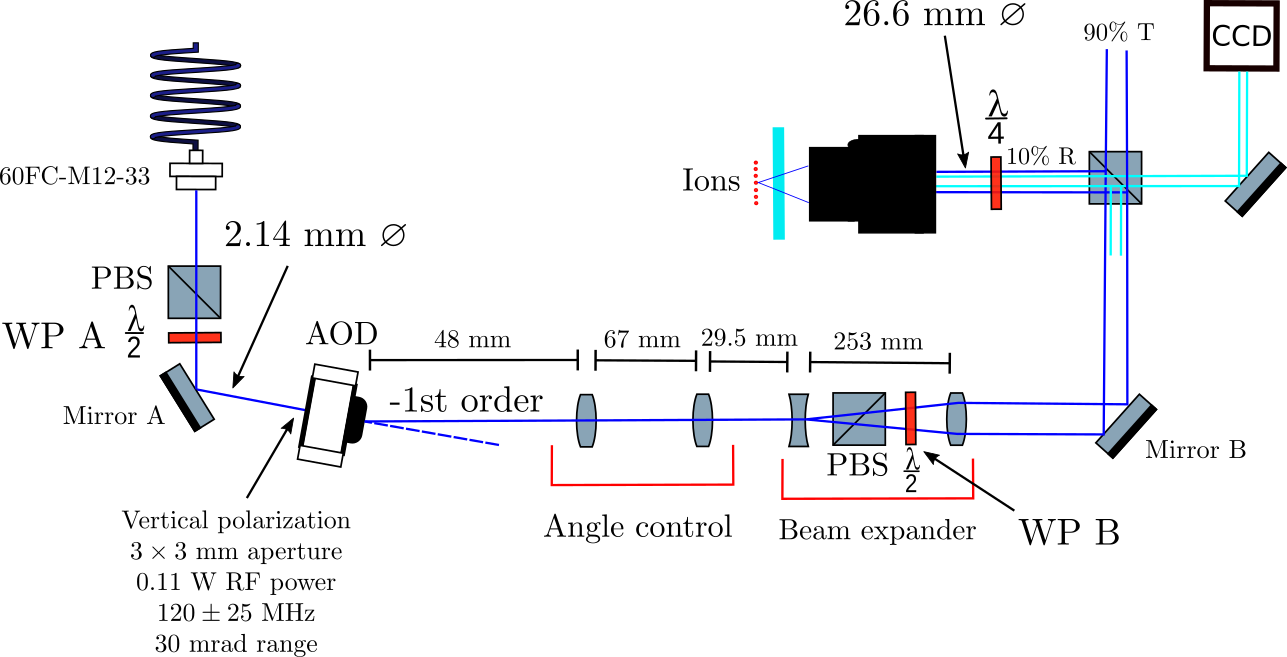
\includegraphics[width=\textwidth]{img/setup}
\caption{Setup scheme}
\end{figure}
\subsubsection{Simulation}

\begin{figure}[H]
\centering
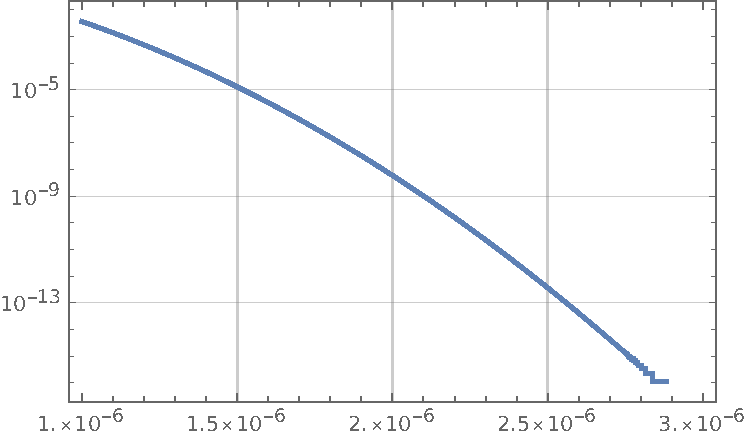
\includegraphics[width=\textwidth]{img/Plosses}
\caption{Losses on the compensation electrodes vs beam waist}
\end{figure}
\begin{figure}[H]
\centering
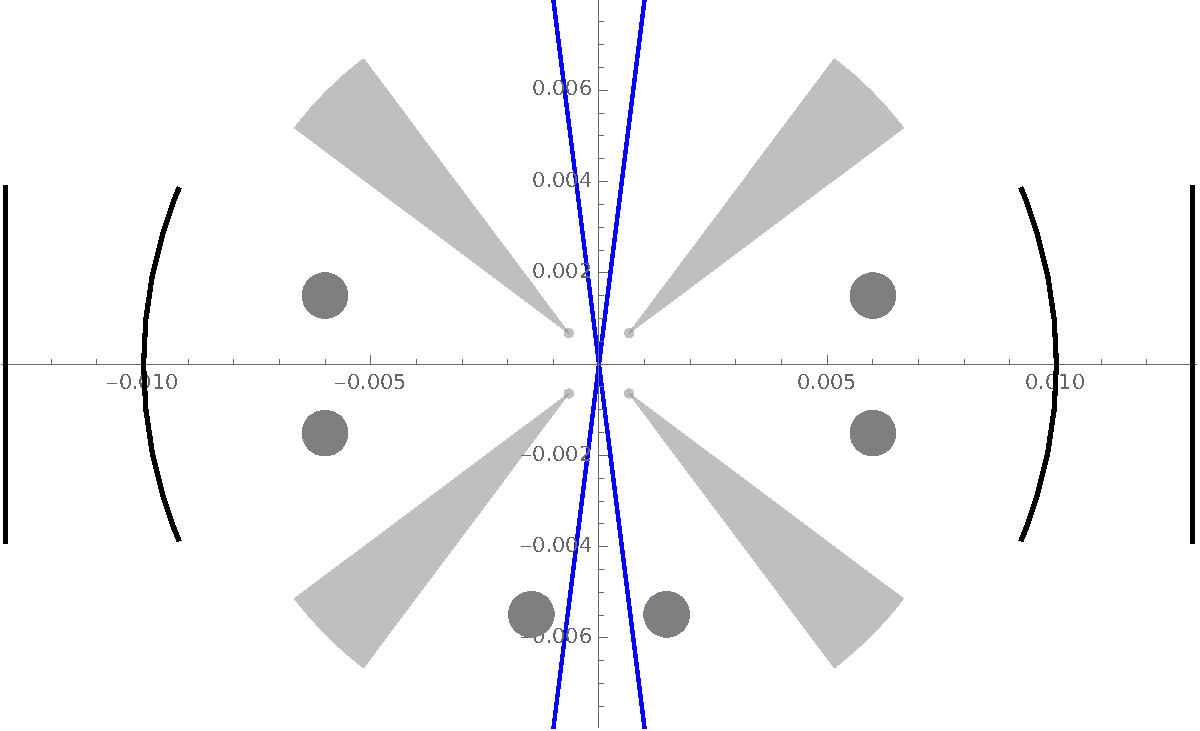
\includegraphics[width=\textwidth]{img/clipping}
\caption{Clipping on compensation electrodes}
\end{figure}

\section{Experimental system}
\subsection{Ion trap and key techniques}
\subsubsection{Calcium Ions}
- Calcium level scheme basically
\subsubsection{Trapping, cooling, and state readout}
- How this stuff is implemented
\subsubsection{Photon generations}
- Cavity enhanced Raman transition
\subsection{Addressing setup}
- Scheme of real setup \\
- Alignment process


\subsubsection{AOD}
\begin{figure}[H]
\centering
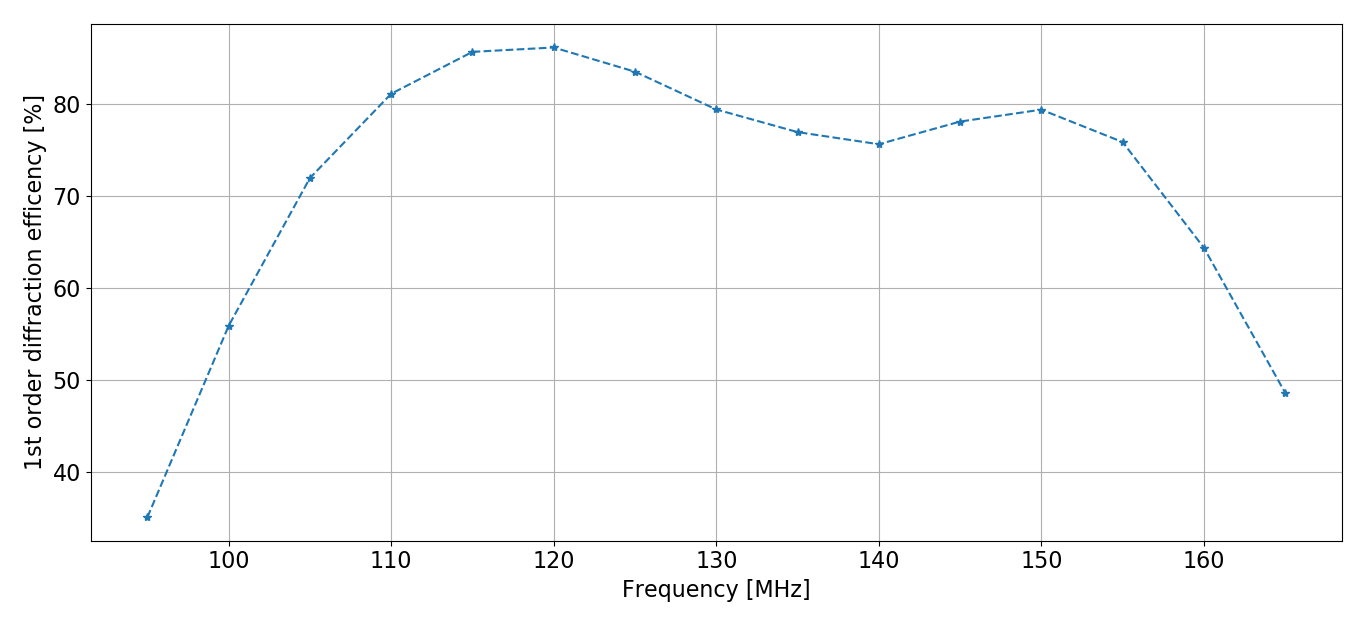
\includegraphics[width=\textwidth]{img/DE}
\caption{AOD diffraction efficency}
\end{figure}

\begin{figure}[H]
\centering
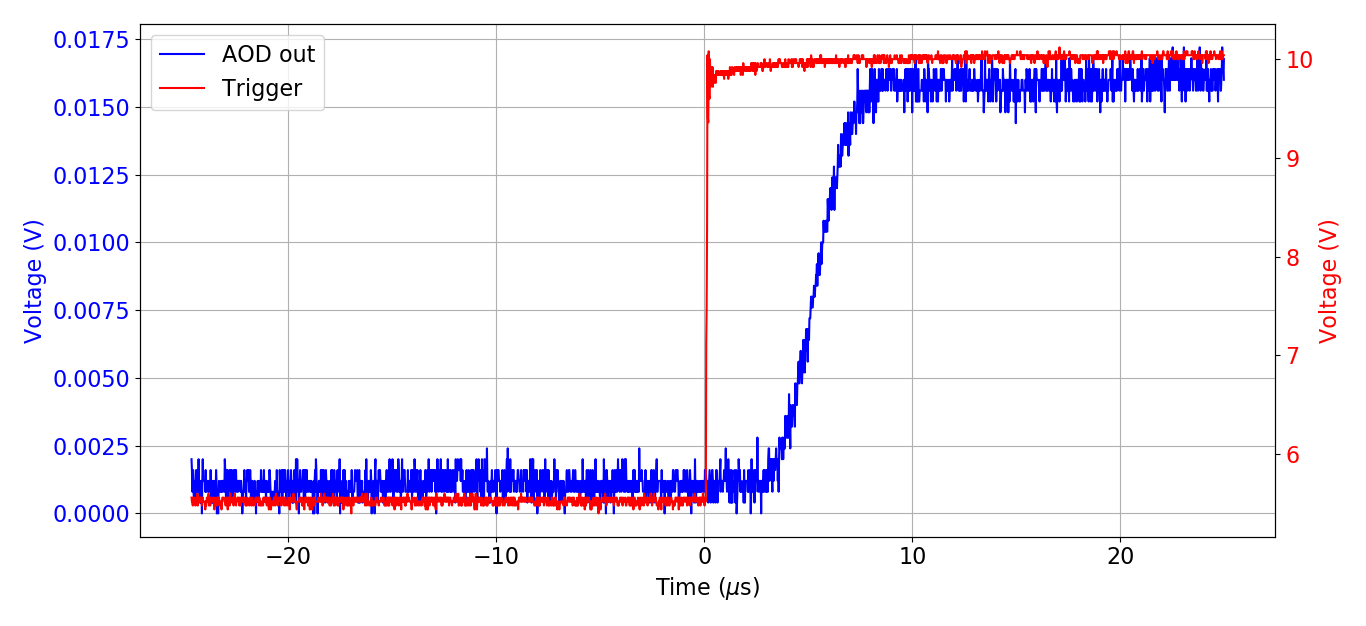
\includegraphics[width=\textwidth]{img/response}
\caption{AOD switching time}
\end{figure}


\section{Results}
\subsection{Test: razor blade and camera}
\begin{figure}[H]
\centering
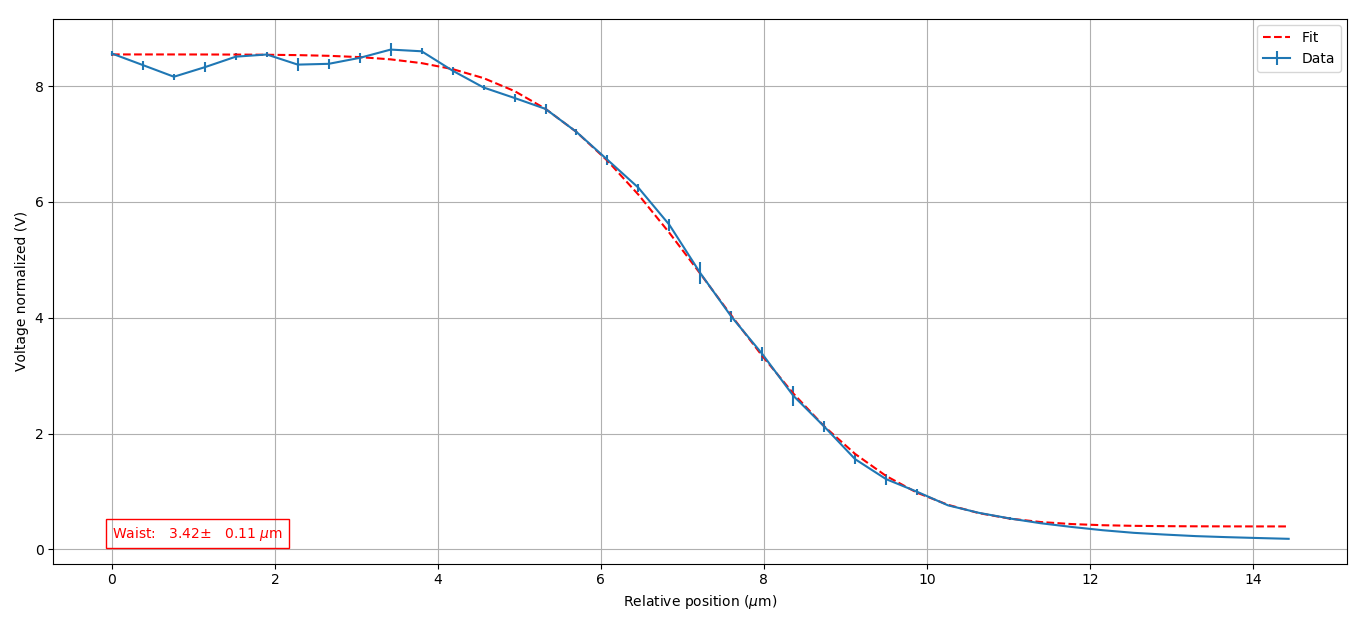
\includegraphics[width=\textwidth]{img/prova7}
\caption{Example of razor scan}
\end{figure}
\begin{figure}[H]
\centering
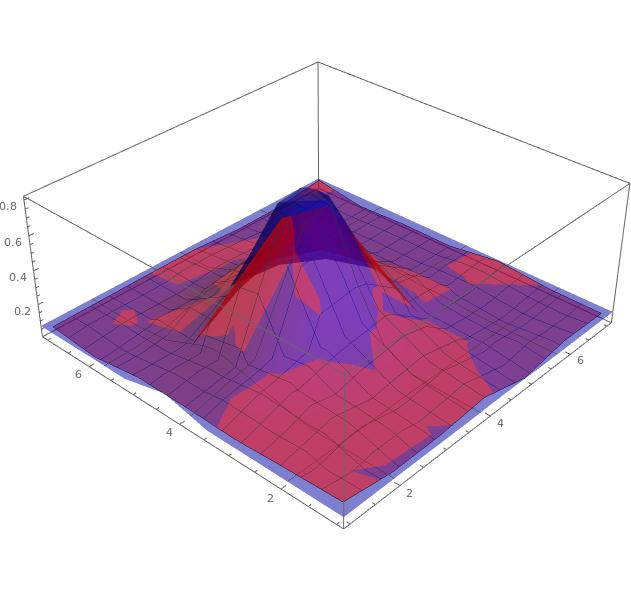
\includegraphics[width=\textwidth]{img/camera}
\caption{Example of camera picture}
\end{figure}
\subsection{Ramsey interferometry}
\begin{figure}[H]
\centering
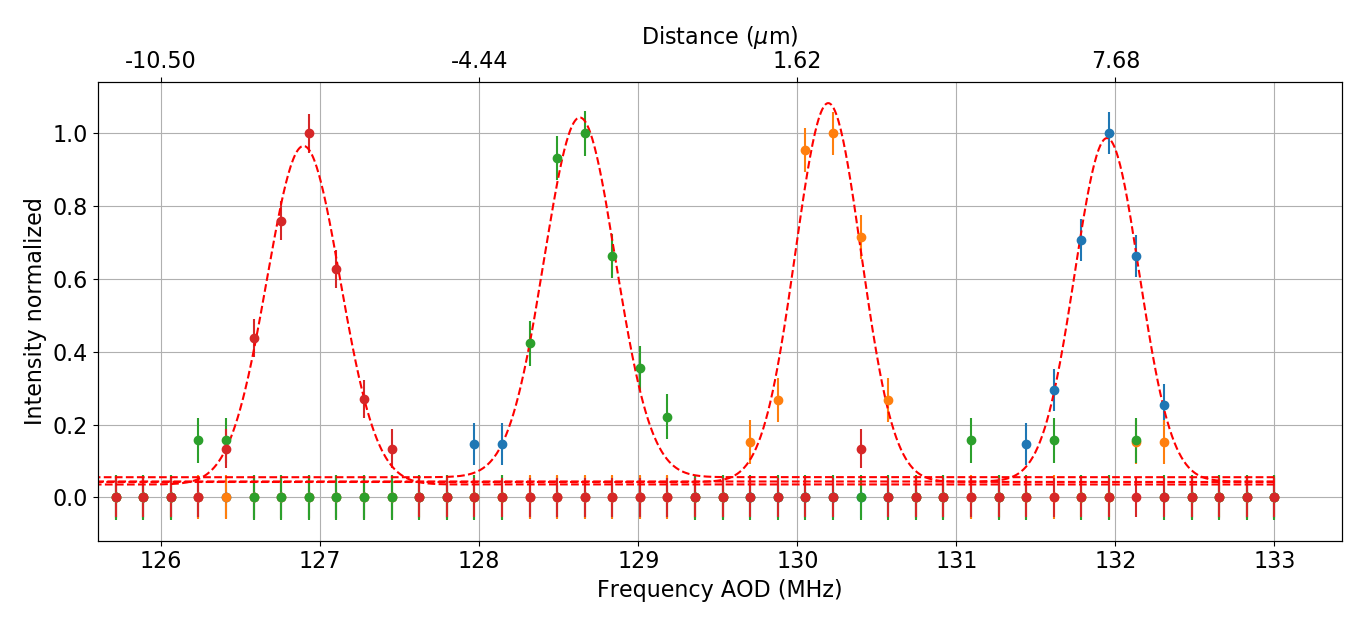
\includegraphics[width=\textwidth]{img/AODscan}
\caption{3 ions scanned}
\end{figure}
\begin{figure}[H]
\centering
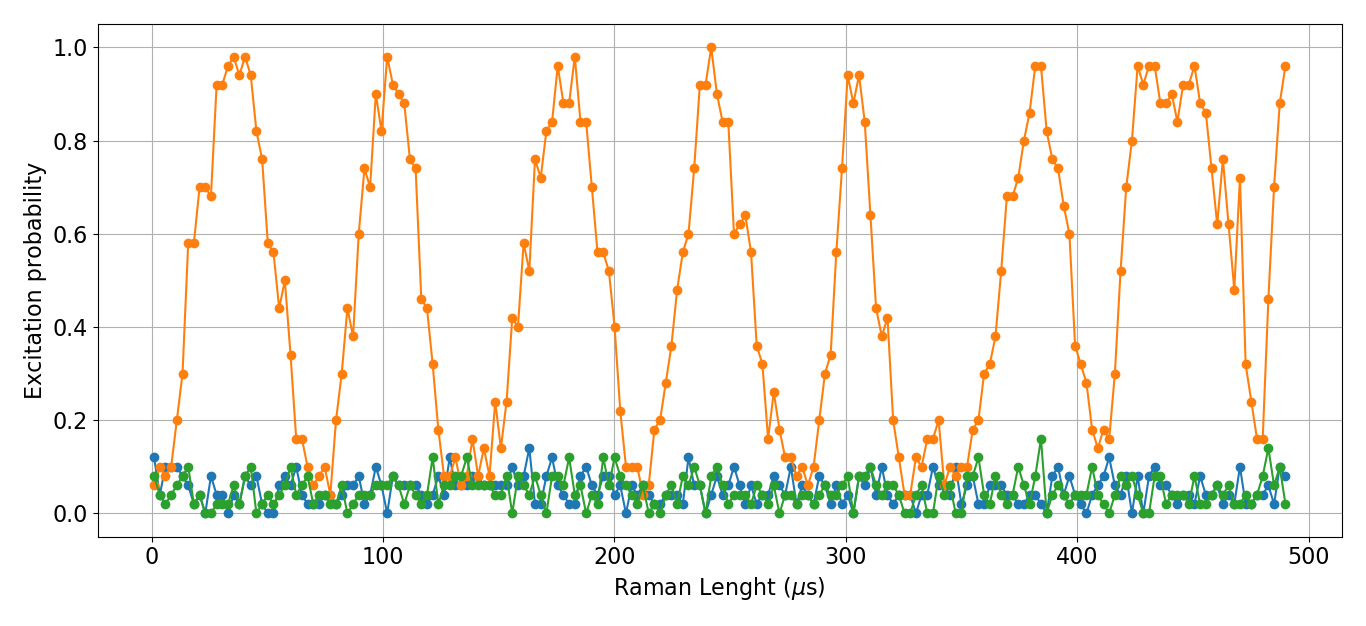
\includegraphics[width=\textwidth]{img/ac_stark}
\caption{393nm AC-Stark flops}
\end{figure}

\subsection{Photons production}
\begin{figure}[H]
\centering
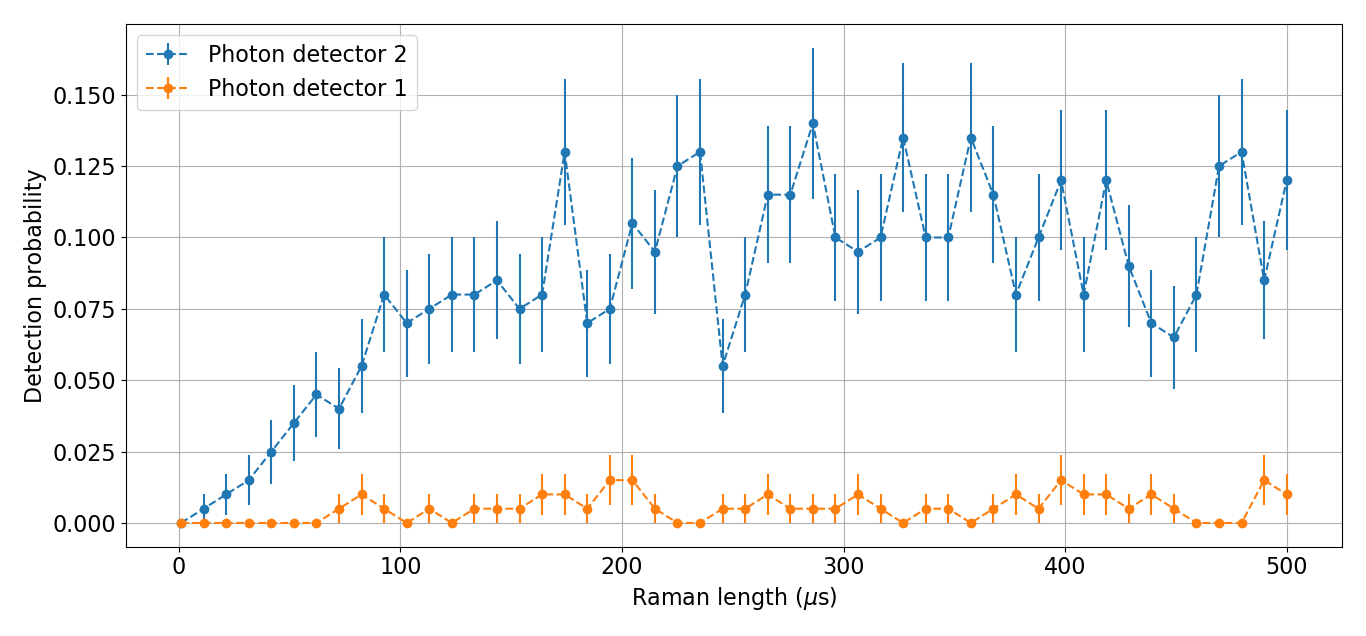
\includegraphics[width=\textwidth]{img/photonefficency_witherror}
\caption{Generated photon efficency}
\end{figure}

\begin{figure}[H]
\centering
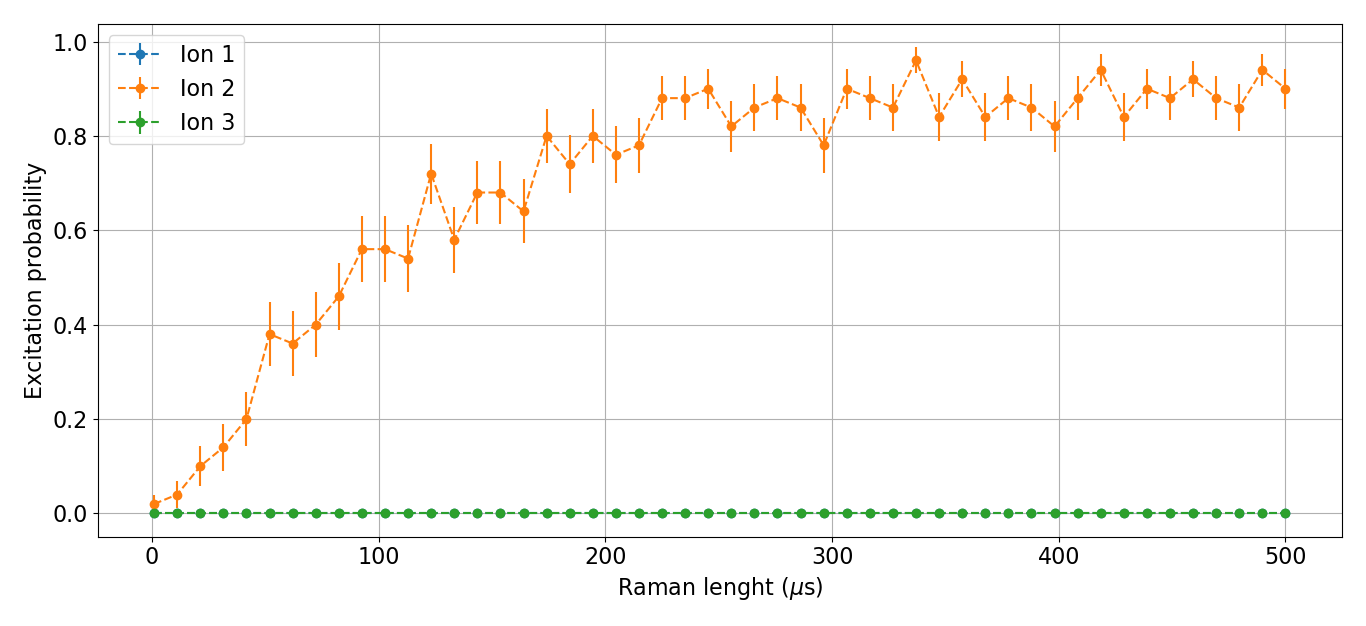
\includegraphics[width=\textwidth]{img/ramanlength_witherrors}
\caption{Excitation of ion while emitting photon}
\end{figure}

- g2 plot?
\section{Conclusions and outlook}
- Usual conclusions

\newpage
%\renewcommand\refname{References} % name for the reference list

\addcontentsline{toc}{section}{References} % to change the name of the references in the TOC
\bibliographystyle{plain}
\bibliography{References} % adds the references to the document


\newpage
\renewcommand{\appendixpagename}{Appendix} % Heading of appendix
\renewcommand{\appendixtocname}{Appendix} % name of appendix in TOC
\appendixpage
\addappheadtotoc


\begin{appendices}
- Error analysis? Maximum likehood estimation?
\end{appendices}

\end{document}
